\section{Cruscotto di valutazione della qualità}
\subsection{Qualità di processo}
\subsubsection{MPC01-EAC (Estimated at Completition)}
\begin{figure}[H]
  \centering
  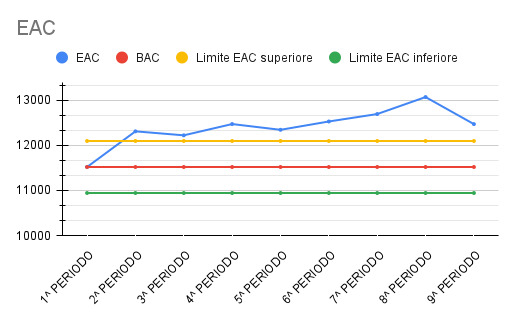
\includegraphics[width=0.7\linewidth]{grafici/EAC.png}
  \caption{Estimated at Completition}
\end{figure}
\textbf{RTB}: Dal grafico si può notare che l'EAC supera il valore accettabile, questo a causa di una scorretta divisione tra ore produttive e individuali, oltre che a lunghi periodi di tempo impiegati nello studio delle $\textit{tecnologie}_G$ necessarie per lo svolgimento del progetto. Si può notare un andamento finale decrescente, quindi si ritiene che dopo la fase iniziale, il gruppo possa rientrare nei valori ottimali. Infine il team è consapevole che l'andamento iniziale del valore è dovuto ad una gestione errata del progetto e quindi i membri dovranno impegnarsi per rientrare nel valore ottimale e garantire il raggiungimento degli obiettivi fissati. \\
\textbf{PB}: Dal grafico si può notare che, durante la fase $\textit{PB}_G$ (decimo periodo in poi), il valore dell'EAC è sceso, rientrando nei valori accettabili. Ciò è dovuto ad una migliore divisione e assegnazione delle tasks e una valutazione del tempo di lavoro più precisa.

\subsubsection{MPC02-PV (Planned Value) e MPC04-EV (Earned Value)}
\begin{figure}[H]
  \centering
  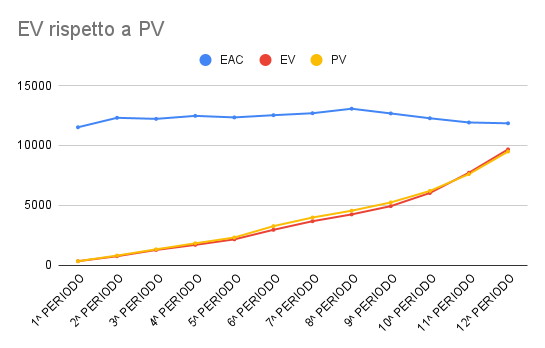
\includegraphics[width=0.7\linewidth]{grafici/EV_PV.png}
  \caption{Planned Value - Earned Value}
\end{figure}
\textbf{RTB}: Dal grafico si può notare che le linee del PV e dell'EV sono molto vicine anche se si può notare un allontanamento dei due valori negli ultimi periodi. Questo denota che il costo preventivato è maggiore del costo sostenuto dal gruppo e quindi il team dovrà impegnarsi maggiormente per terminare le attività stabilite.
\\\textbf{PB}: Si può notare che il valore PV e EV sono molto vicini tra di loro e quindi il costo effettivo rispetta quanto preventivato.
\subsubsection{MPC05-ETC (Estimated to Complete)}
\begin{figure}[H]
  \centering
  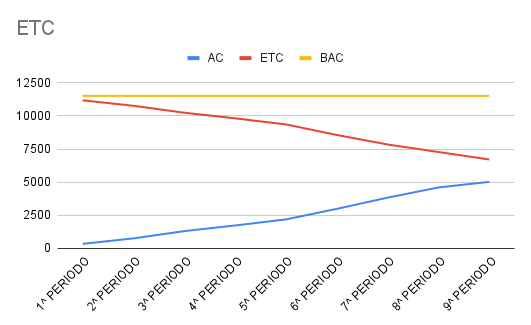
\includegraphics[width=0.7\linewidth]{grafici/ETC.png}
  \caption{Estimated to Complete}
\end{figure}
\textbf{RTB}: Dal grafico si può notare che le linee dell'AC e dell'ETC nel corso dei vari periodi, mantengano un andamento costante. Di conseguenza si può affermare che il progetto stia mantenendo un ritmo regolare di avanzamento. 
\\\textbf{PB}: Dal nono periodo si può notare un incremento dell'andamento del gruppo rispetto al periodo $\textit{RTB}_G$.
\subsubsection{MPC06-CV (Cost Variance), MPC07-SV (Schedule Variance) e MPC08-BV (Budget Variance)}
\begin{figure}[H]
  \centering
  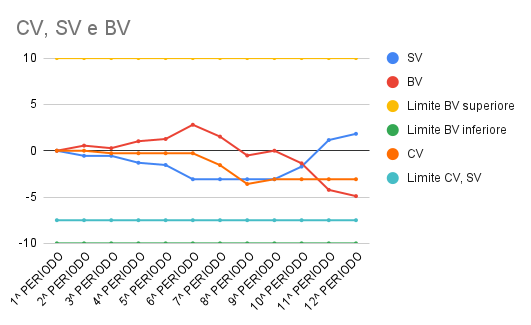
\includegraphics[width=0.7\linewidth]{grafici/CV, SV e BV.png}
  \caption{Cost Variance - Schedule Variance - Budget Variance}
\end{figure}
\textbf{RTB}: Dal grafico si può notare che la linea della Cost Variance ha mantenuto un andamento costante e lineare fino al sesto periodo, cosa positiva. Dal settimo periodo periodo però c'è stato un calo, ciò si può ricondurre alla quasi assente divisione delle ore produttive da quelle individuali. Osservando la Schedule Variance si nota invece che l'allontanamento dal valore preferibile è iniziato molto prima. Questa situazione è stata causata da un misto di mancata divisione delle ore produttive e ore individuali, e di sottostime delle ore da dare per ogni lavoro. Infine, osservando la Budget Variance, si nota che, nonostante si sia speso più di quanto previsto per la maggior parte del tempo, ciò si è stabilizzato negli ultimi periodi.\\
\textbf{PB}: Durante la $\textit{PB}_G$ (decimo periodo in poi) si nota un abbassamento della BV, con un aumento della SV; questo è dato dal fatto che durante questa fase il gruppo ha saputo gestire meglio le task. Nonostante ciò, i valori rientrano all'interno dei limiti imposti dal gruppo stesso. Per quanto riguarda la Cost Variance, si nota un calo e una stabilizzazione verso la fine; questo a causa di molte task implementative che hanno richiesto un tempo di completamento maggiore e quindi un costo maggiore rispetto a quanto preventivato inizialmente.
%\subsection{MPC09-RSI (Requirements stability index)}
%\subsection{MPC14-IG (Indice Gulpeanse)}
\subsubsection{MPC09-RSI (Requirements stability index)}
Per quanto riguarda l'attinenza dell'inquadramento dei requisiti funzionali del progetto, un incontro avuto nel corso del 10° periodo con l'azienda proponente ha portato a una importante revisione di quelli che erano stati individuati come "requisiti obbligatori" nel corso della fase $\textit{RTB}_G$. A causa di ritardi nello sviluppo, infatti, e al fine di non sforare con la data di consegna prefissata, il gruppo ha concordato insieme al proponente di definire alcuni requisiti, precedentemente individuati come "obbligatori", "desiderabili". Nonostante dunque l'elevato numero di requisiti che hanno richiesto una revisione nel corso della $\textit{PB}_G$, il \textit{Requirements stability index} risulta comunque superiore al valore accettabile. 
\begin{center}
    \begin{tabular}{|p{3cm}|p{4cm}|p{3cm}|p{3cm}|p{3cm}|}
    \hline
    \textbf{Metrica} & \textbf{Nome} & \textbf{Valore \newline accettabile} & \textbf{Valore \newline ottimale} & \textbf{Valore \newline ottenuto} \\
    \hline
    MPC09-RSI & \textit{Requirements stability index} & 70\% & 100\% & 72\% \\
    \hline
    \end{tabular}
\end{center}
% TO DO
\subsubsection{MPC15-PCTS (Percentuale dei test superati)}
Per quanto riguarda la percentuale dei $\textit{test}_G$ superati, dal momento della loro introduzione nel corso del 10° periodo, il loro superamento è sempre stato verificato prima dell'effettivo \textit{merge} all'interno del $\textit{branch}_G$ \textit{develop}. A parte dunque per un primo periodo in cui non era ancora completata appieno l'automazione di \textit{$\textit{test}_G$ coverage} all'interno del \textit{repository}, si è sempre ottenuto una percentuale di $\textit{test}_G$ superati pari al 100\%, valore che corrisponde a quello ottenuto con la build definitiva. 
\begin{center}
    \begin{tabular}{|p{3cm}|p{4cm}|p{3cm}|p{3cm}|p{3cm}|}
    \hline
    \textbf{Metrica} & \textbf{Nome} & \textbf{Valore \newline accettabile} & \textbf{Valore \newline ottimale} & \textbf{Valore \newline ottenuto} \\
    \hline
    MPC15-PCTS & Percentuale dei $\textit{test}_G$ superati & 80\% & 100\% & 100\% \\
    \hline
    \end{tabular}
\end{center}
\subsubsection{MPC16-SC (Statement Coverage)}
La \textit{Statement Coverage} misura la percentuale di istruzioni eseguite durante l'esecuzione dei $\textit{test}_G$. Si calcola come il numero di istruzioni eseguite almeno una volta rispetto al totale di istruzioni nel programma. \\
Il suo scopo è assicurarsi che tutte le istruzioni nel codice vengano testate almeno una volta. \\
Di seguito si riporta un grafico rappresentate la percentuale di \textit{Statement Coverage} relativa a quelle che \textit{Coveralls} considera come "\textit{relevant lines}", per ciascun file contenente codice coperto da $\textit{test}_G$. 
\begin{figure}[H]
    \centering
    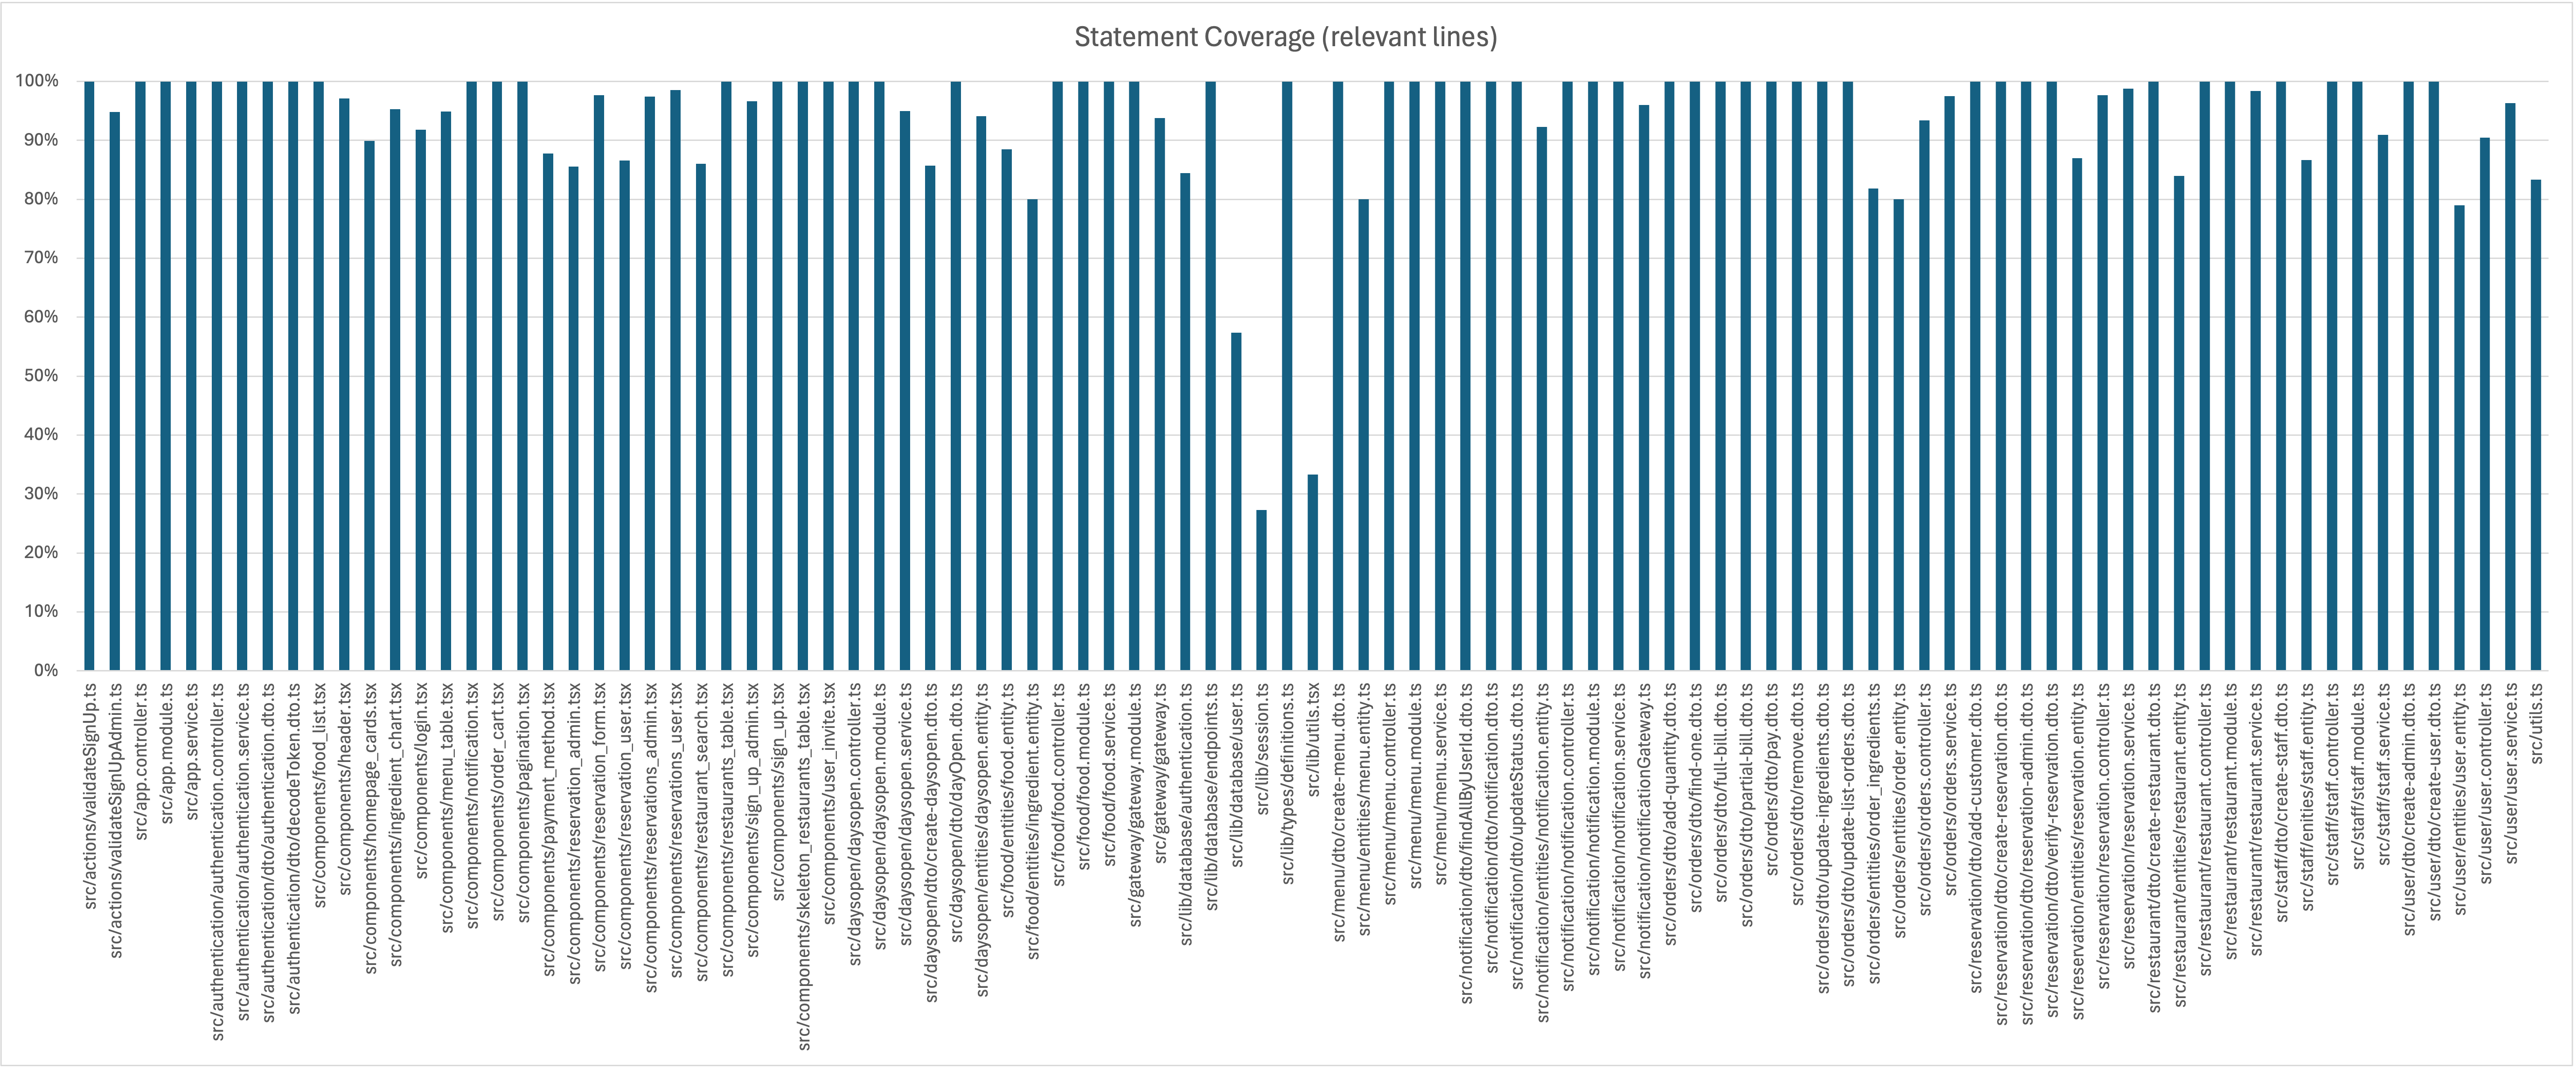
\includegraphics[scale = 0.4]{grafici/Statement_Coverage.png}
    \caption{\textit{Statement Coverage}}
\end{figure}
% TO DO
\subsubsection{MPC17-BC (Branch Coverage)}
La \textit{Branch Coverage} misura la percentuale di rami eseguiti all'interno delle strutture di controllo durante l'esecuzione dei $\textit{test}_G$. \\
Il suo scopo è assicurare che ogni possibile percorso logico all'interno del codice il codice sia stato testato almeno una volta. \\
Di seguito si riporta un grafico rappresentate la percentuale di \textit{Branch Coverage} relativa a tutti quei file che contengono codice in cui sono presenti rami e che sono stati coperti da $\textit{test}_G$. 
\begin{figure}[H]
    \centering
    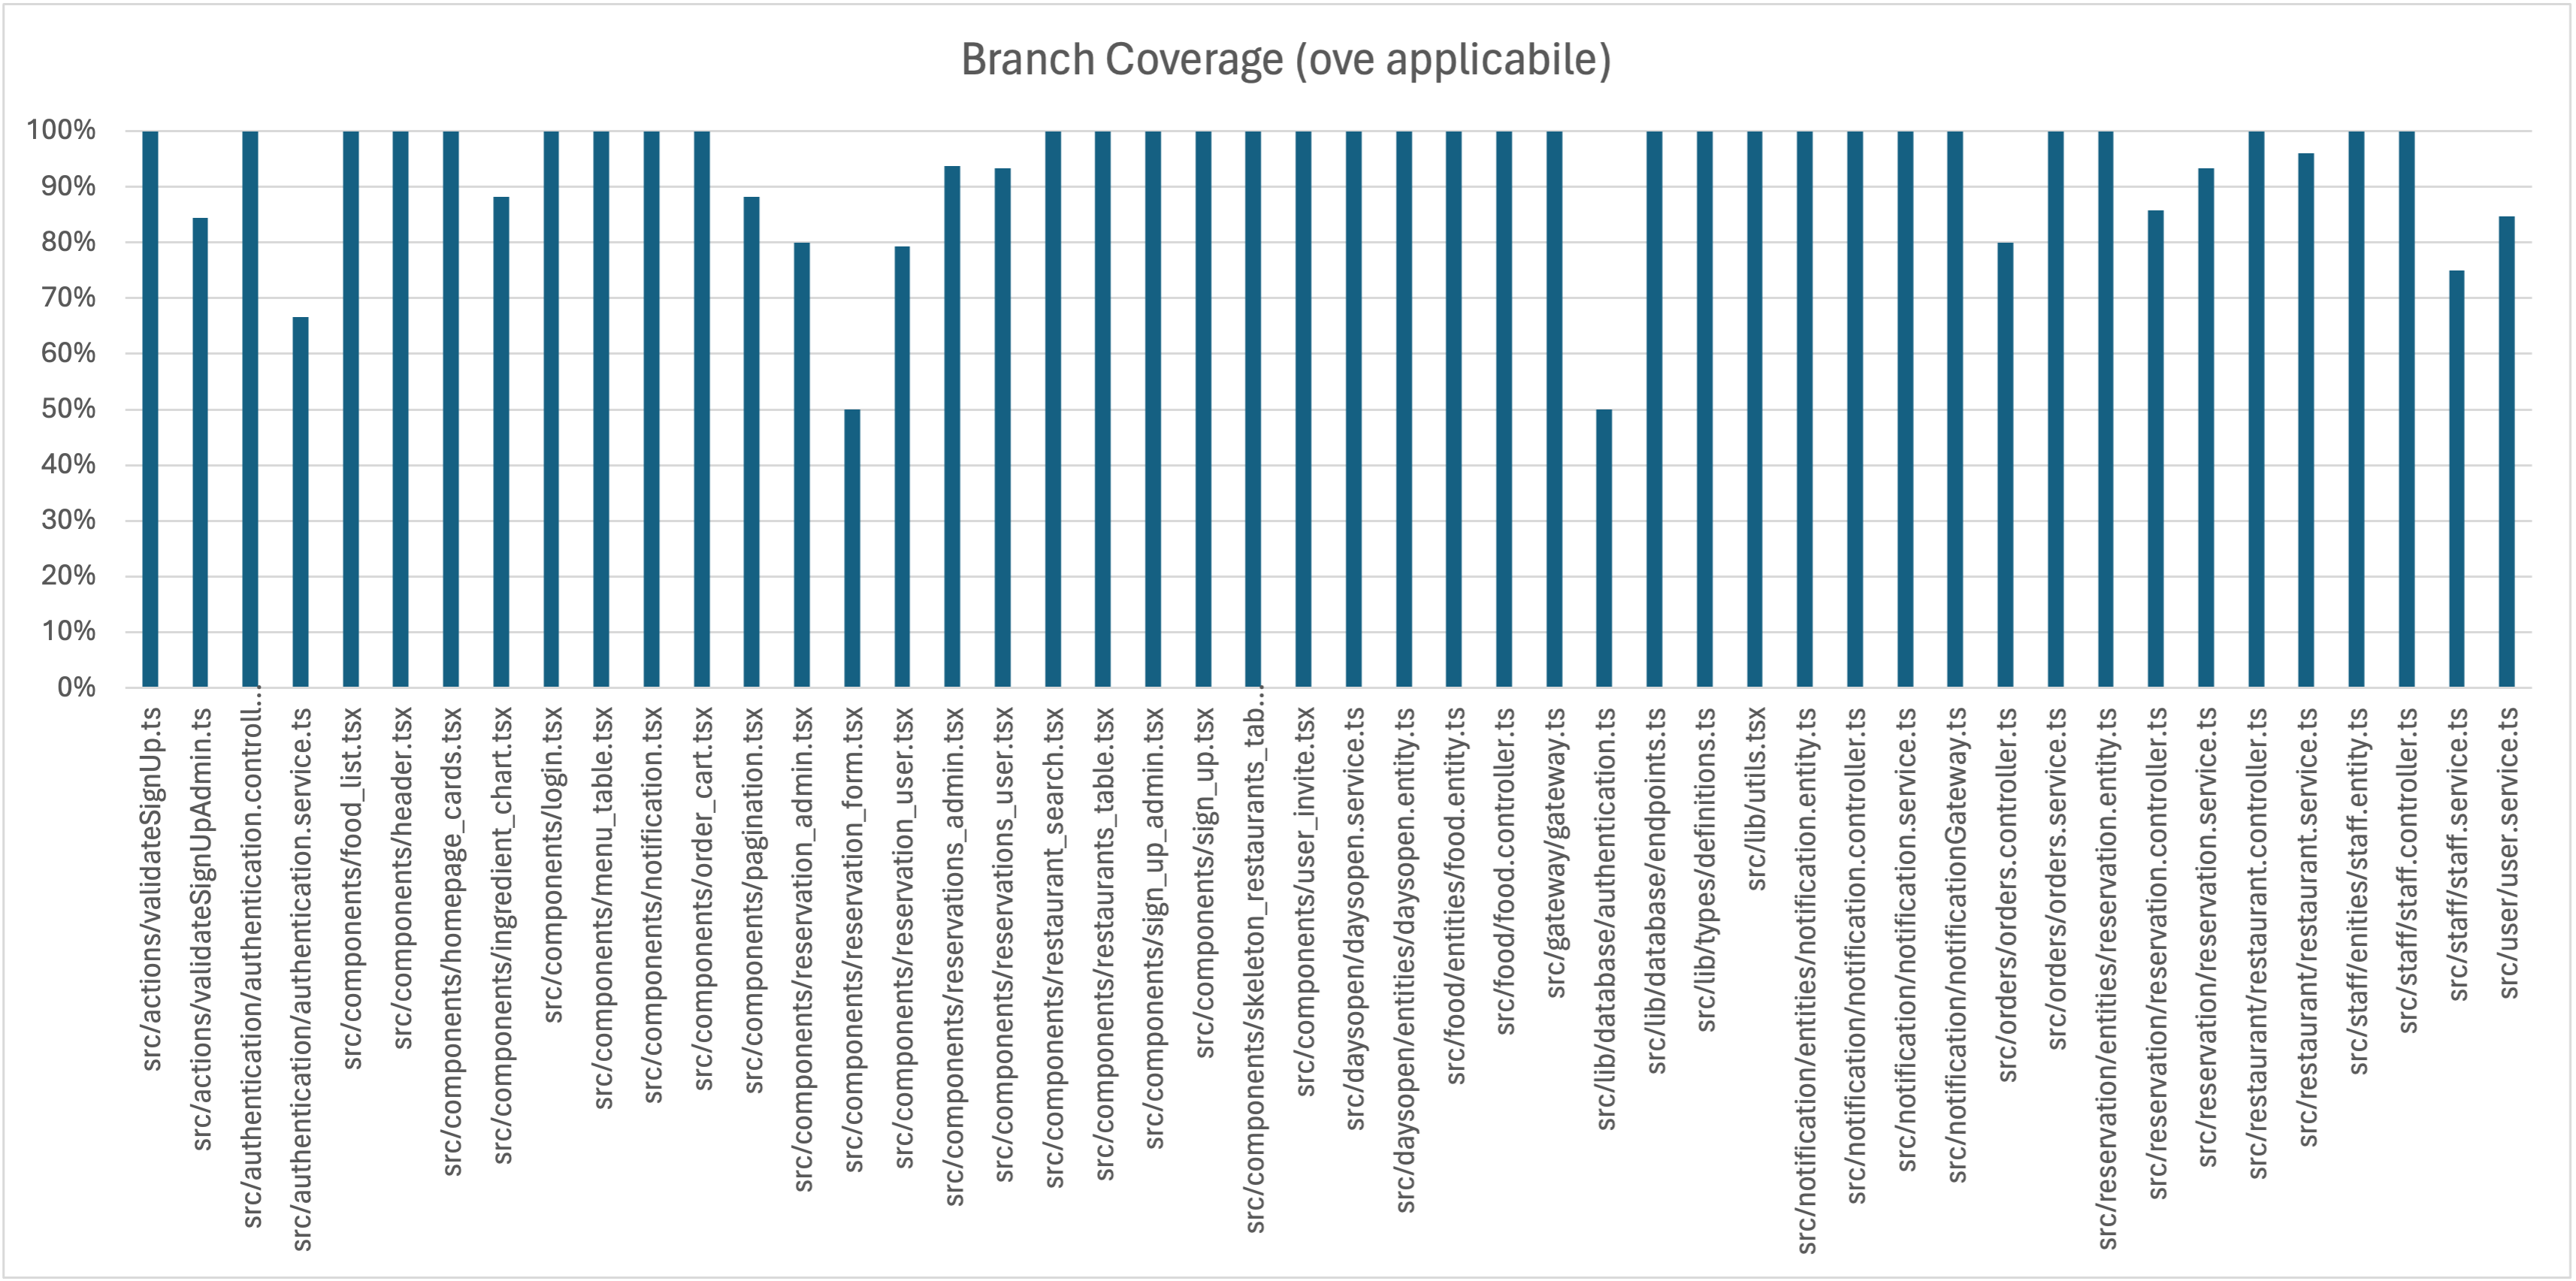
\includegraphics[scale = 0.6]{grafici/Branch_Coverage.png}
    \caption{\textit{Branch Coverage}}
\end{figure}
% TO DO
\subsubsection{MPC19-NCR (Non Calculated Risk)}
\begin{figure}[H]
  \centering
  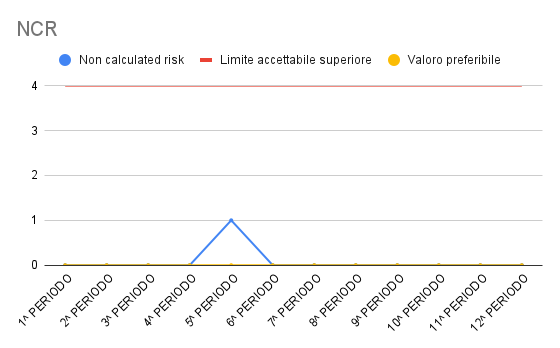
\includegraphics[width=0.7\linewidth]{grafici/NCR.png}
  \caption{Non Calculated Risk}
\end{figure}
Dal grafico si può notare che per la maggior parte del tempo non sono comparsi $\textit{rischi}_G$ non previsti. Solo nel quinto periodo è emerso un rischio di cui non si era tenuto conto inizialmente, ovvero la sessione di esami, la quale ha portato via parecchio tempo ai vari membri del gruppo, rallentando di molto l'avanzamento del lavoro.
%\subsection{MPC16-ET (Efficienza temporale)}
\subsection{Qualità di prodotto}
\subsubsection{MPD01-CRO (Copertura dei requisiti obbligatori)}
Il numero di requisiti obbligatori è stato ridotto a seguito di un colloquio avuto con il proponente nel 10° periodo. La necessità di ridurre il numero di requisiti obbligatori è stata dettata dal ritardo accumulato dal gruppo nel corso dello sviluppo del \textit{software}. Al termine dell'11° periodo sono stati soddisfatti tutti i requisiti obbligatori individuati. 
\begin{center}
    \begin{tabular}{|p{3cm}|p{4cm}|p{3cm}|p{3cm}|p{3cm}|}
    \hline
    \textbf{Metrica} & \textbf{Nome} & \textbf{Valore \newline accettabile} & \textbf{Valore \newline ottimale} & \textbf{Valore \newline ottenuto} \\
    \hline
    MPD01-CRO & Copertura dei requisiti obbligatori & 100\% & 100\% & 100\% \\
    \hline
    \end{tabular}
\end{center}

\begin{comment}
\subsubsection{MPD02-CRD (Copertura dei requisiti desiderabili)}
A seguito di un colloquio avuto con il proponente avvenuto nel 10° periodo, alcuni requisiti obbligatori sono stati convertiti in requisiti desiderabili per le medesime ragioni descritte nel punto di cui sopra. Al termine dell'11° periodo sono stati soddisfatti tutti i requisiti desiderabili che il gruppo è riuscito ad integrare nel progetto \textit{software} al fine di rientrare nei tempi di sviluppo concordati, che purtroppo rimangono al di sotto del valore ottimale; la scelta è stata presa al fine di non ritardare ulteriormente la consegna del progetto. 
\begin{center}
    \begin{tabular}{|p{3cm}|p{4cm}|p{3cm}|p{3cm}|p{3cm}|}
    \hline
    \textbf{Metrica} & \textbf{Nome} & \textbf{Valore \newline accettabile} & \textbf{Valore \newline ottimale} & \textbf{Valore \newline ottenuto} \\
    \hline
    MPD02-CRD & Copertura dei requisiti desiderabili & 50\% & 100\% & 11\% \\
    \hline
    \end{tabular}
\end{center}
\end{comment}
\subsubsection{MPC07-FD (Failure Density)}
A seguito del termine dello sviluppo \textit{software}, per quanto riguarda il completamento dei $\textit{test}_G$, il gruppo ha ottenuto una percentuale di successo di completamento dei $\textit{test}_G$ pari al 100\%. \\
Nel corso dei vari \textit{merge} nel $\textit{branch}_G$ \textit{develop}, calcolati a partire dal 10° periodo (periodo durante il quale sono stati inizialmente inseriti dei \textit{$\textit{test}_G$}), solo in una prima fase in cui non era completata l'automazione di \textit{$\textit{test}_G$ coverage} si registra un elevato numero di $\textit{test}_G$ falliti, arrivando comunque a un totale di solo 20 su 54 \textit{merge} che abbiano dato come esito "\textit{fail}". Ciò è verificabile andando a controllare la sezione "Code Coverage" della $\textit{repository}_G$ GitHub.
\begin{center}
    \begin{tabular}{|p{3cm}|p{4cm}|p{3cm}|p{3cm}|p{3cm}|}
    \hline
    \textbf{Metrica} & \textbf{Nome} & \textbf{Valore \newline accettabile} & \textbf{Valore \newline ottimale} & \textbf{Valore \newline ottenuto} \\
    \hline
    MPC07-FD & Failure Density & 10\% & 0\% & 0\% \\
    \hline
    \end{tabular}
\end{center}